\section{Testbed}
\label{sec:testbed}
To verify the functionality of the NAT traversing procedure, a testbed was been realized. The structure of the testbed is reported in figure \ref{fig:testbed_structure}.
\begin{figure}[htbp]
	\centering
		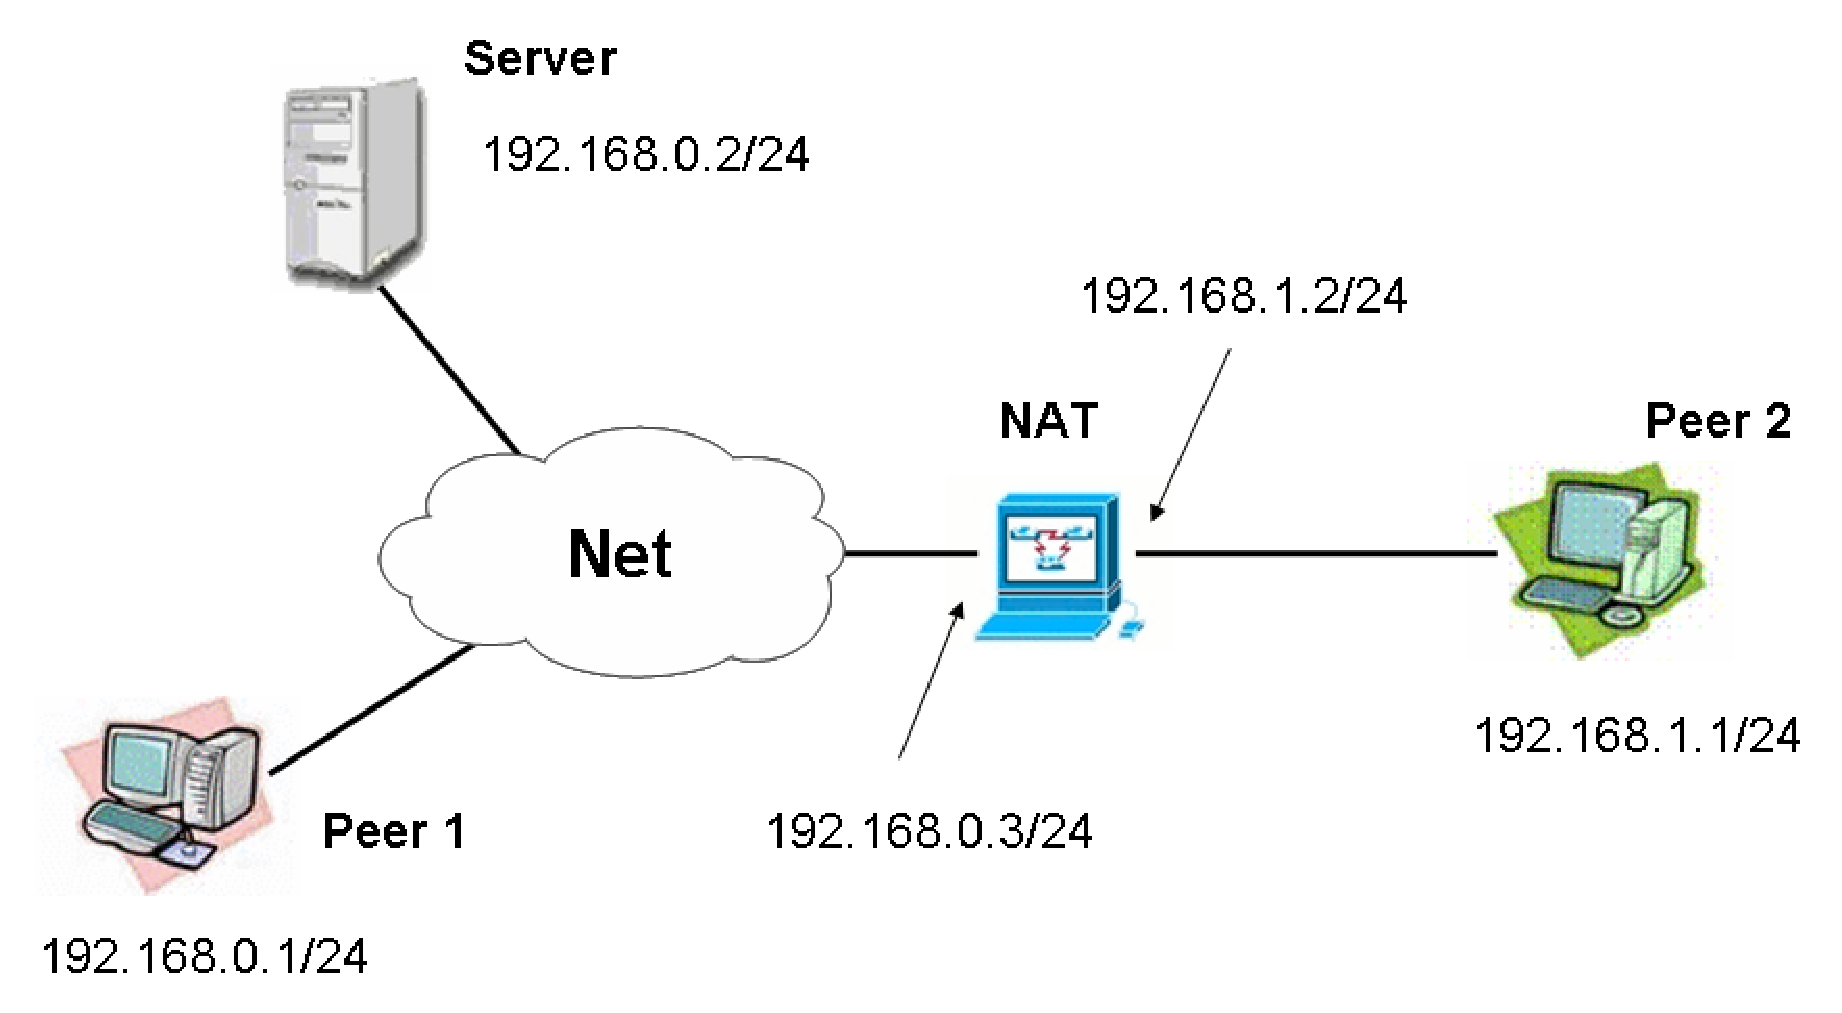
\includegraphics[scale=0.4]{testbed_structure.eps}
	\caption[Structure of the testbed]{Logic structure of the testbed}	
	\label{fig:testbed_structure}
\end{figure}
As it is visible there are two peer (one behind the NAT) and a server.
To test the procedure the first peer to register to the server is that behind the NAT. The second peer than register itself at the server and try to communicate with the other peer. This is possible only if the traversing procedure works good. There are many methods to realize this structure:
\begin{enumerate}
	\item Via hardware: all the devices are real hardware
	\item Hybrid: some devices are hardware and other are simulated via software
	\item Virtual: all the devices are virtual machine
\end{enumerate}
Our approach is the third. The virtualization software is Sun VirtualBox 2.1.4. There are five VM (Virtual Machine): four to realize all the devices and one to control the simulation in a centralized modes. The VMs mount a Linux distribution (Damn Small Linux 2.1).
The structure of the control network is reported in figure \ref{fig:control_network}.
\begin{figure}[htbp]
	\centering
		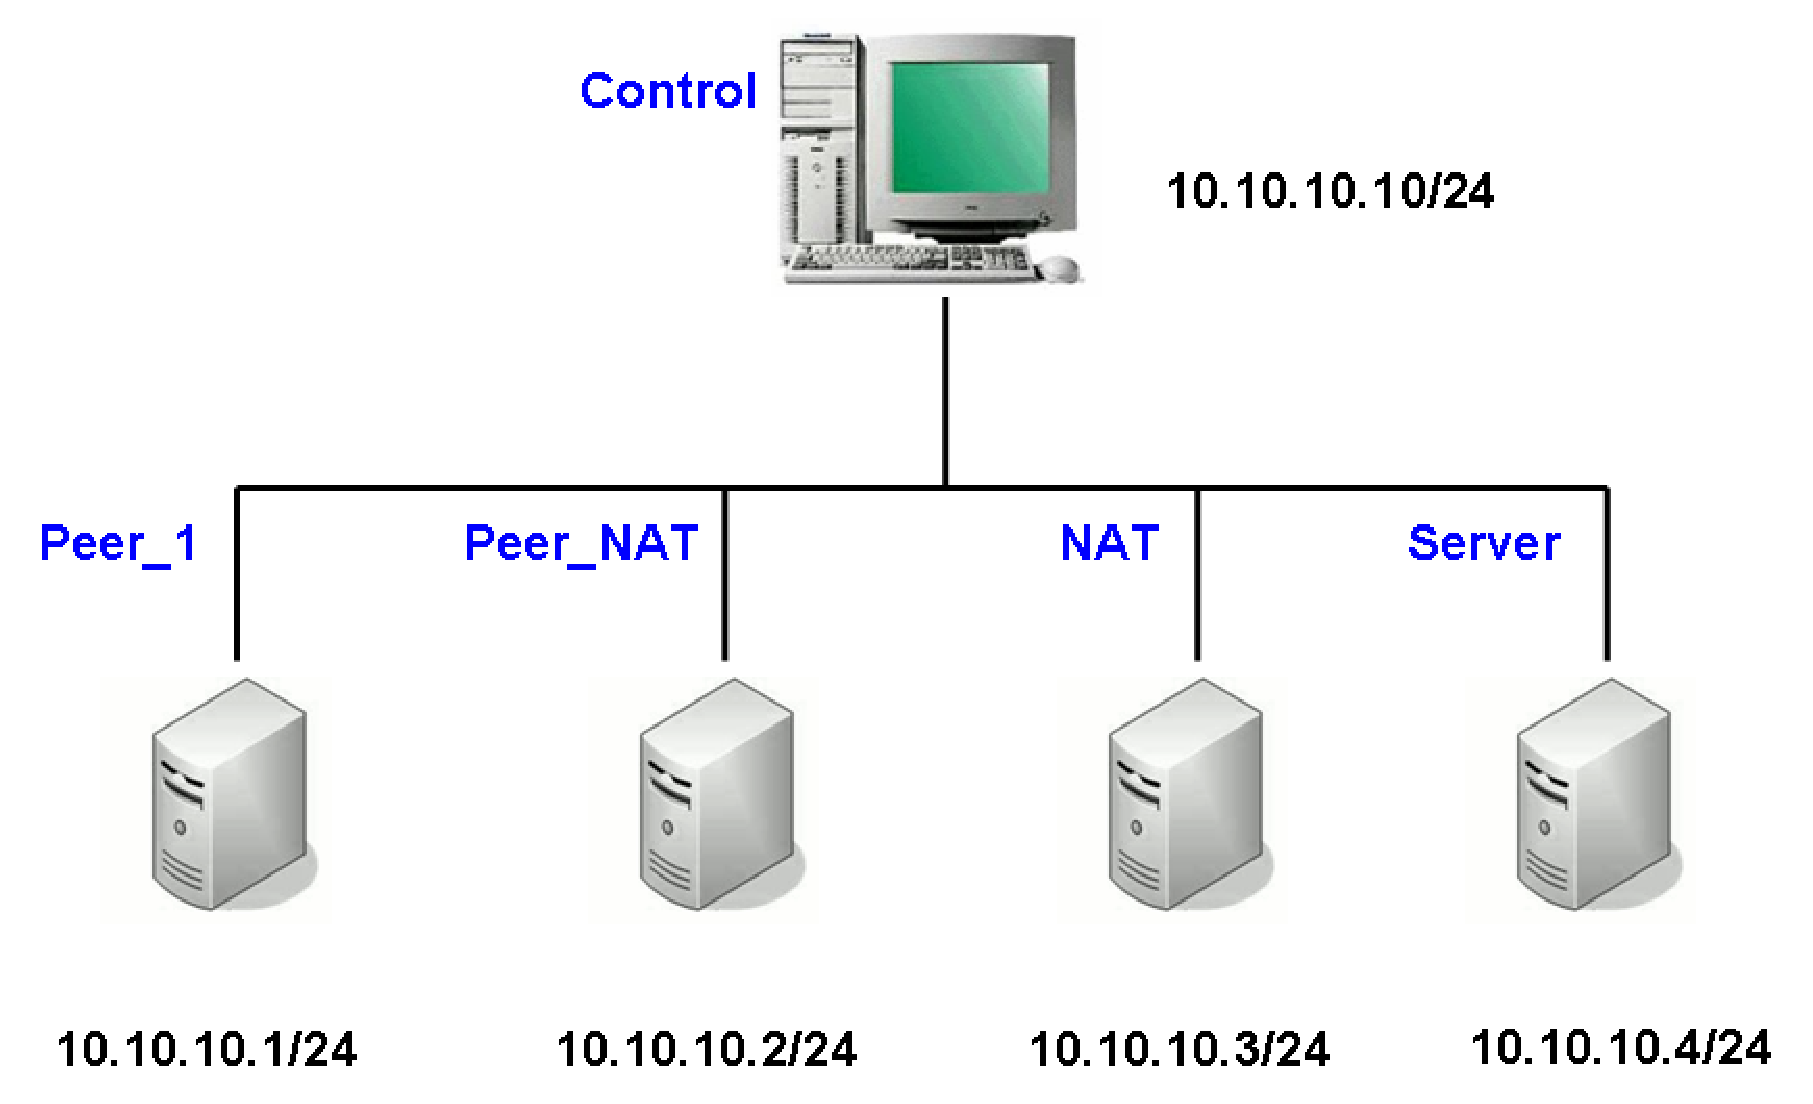
\includegraphics[scale=0.4]{control_network.eps}
	\caption[Testbed Control Network]{Control network of the testbed}
	\label{fig:control_network}
\end{figure}
Every VM is achievable from the Control VM via ssh\footnote{Every VM consider the Control VM as a \emph{known-host} hence the ssh session don't ask for password.}. 
The software is composed by several files:
\begin{itemize}
	\item \textbf{client:} a client that implement a text-based section to communicate with the server for the first phase of the setup and a PPETP section. This file is present in the following VMs: DSL1, DSL2 and DSL\_Server
	\item \textbf{server\_main:} The text-based server, it communicate with the \emph{server-client} for the complete setup. It is placed only in the DSL\_Server
	\item \textbf{server\_config.xml:} A configuration file used to setup the \emph{server-client}. This file is placed only in the DSL\_Server
	\item \textbf{execute\_server.sh:} This file start the \emph{server\_main} and the \emph{server\_client}. It is present only in the DSL\_Server
	\item \textbf{execute\_client.sh:} This file start a client. It is placed in the DSL2 and the DSL\_Server
	\item \textbf{execute\_client\_test.sh:} This file start a client and wait for the result of the test to verify the hole on the NAT
	\item \textbf{nat\_config.sh:} This file is used to setup the NAT configuration
\end{itemize}  
The following tables summarize the allocation of the files on the VMs
\begin{figure}[htbp]
	\centering
		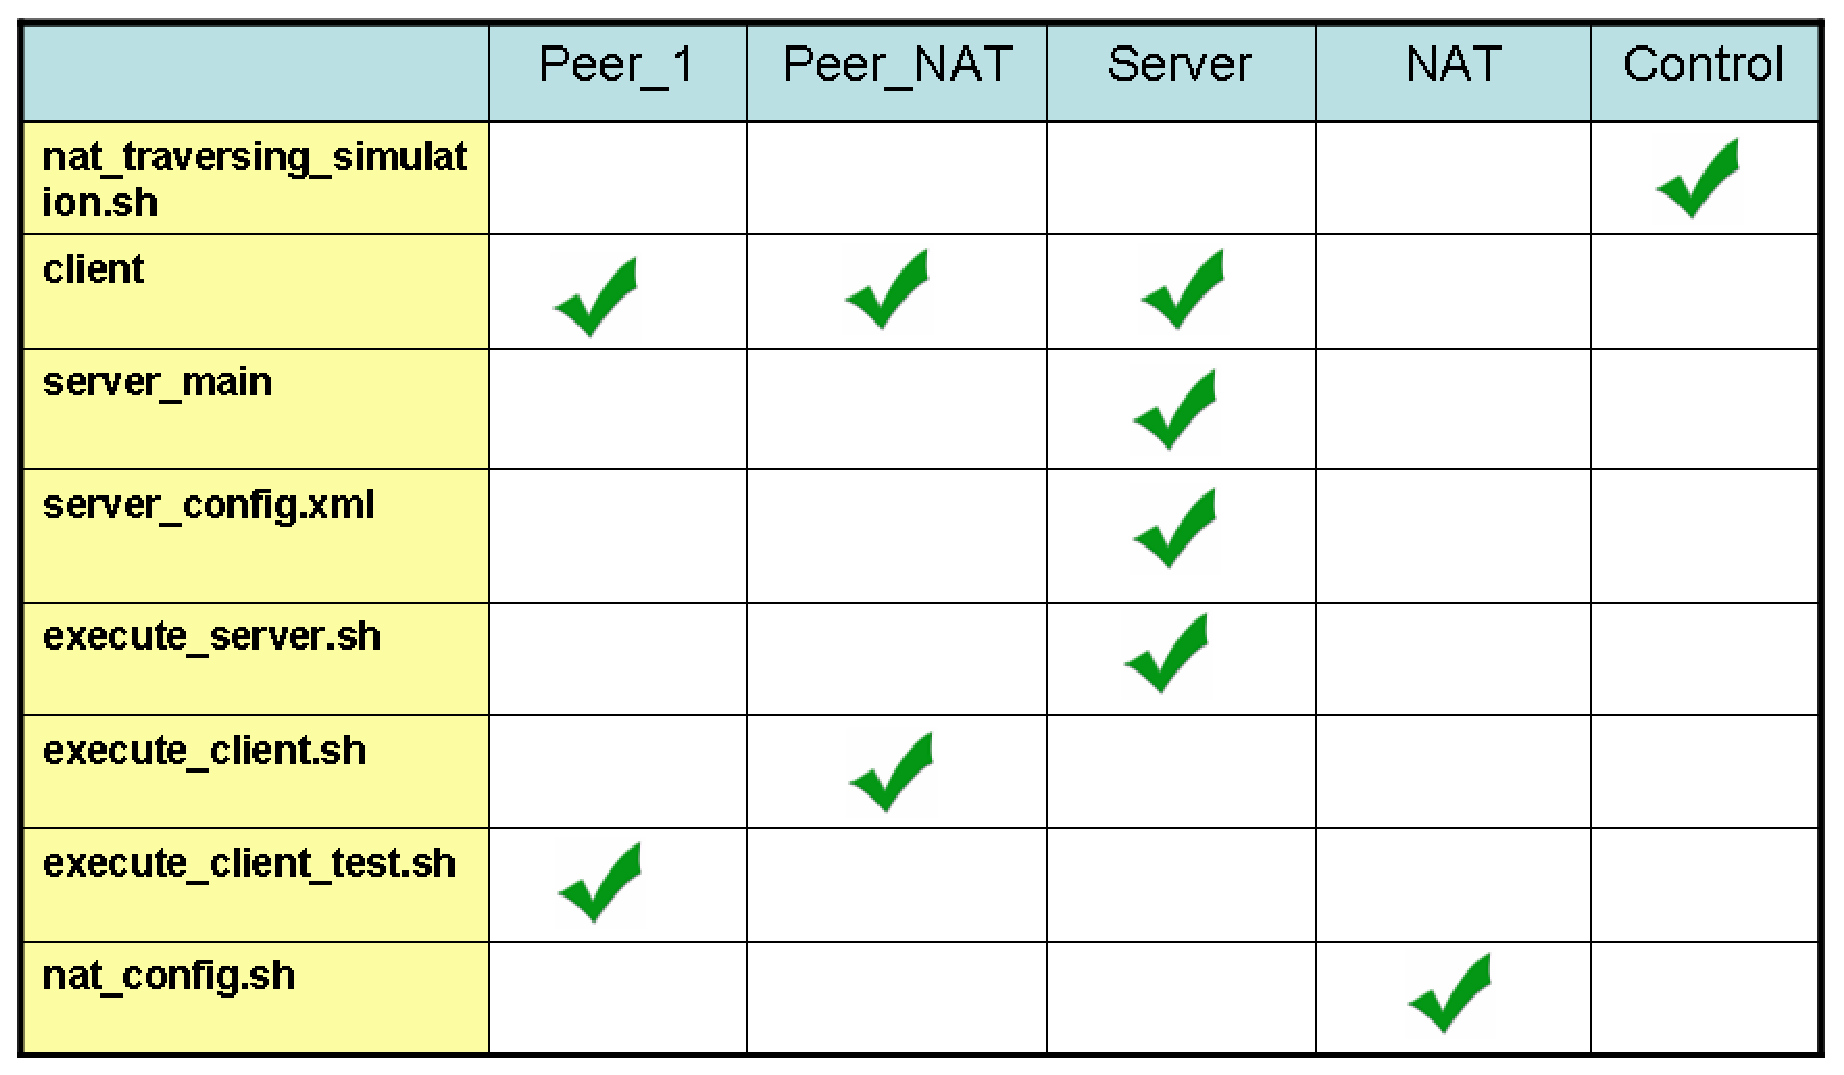
\includegraphics[scale=0.4]{files_table.eps}
	\caption[File allocation]{Allocation of the files on the VMs}	
	\label{fig:files_table}
\end{figure}
%
As you can see in the table, in the server VM there are both the server and the client programs. This is necessary because the \emph{server\_main} doesn't ``speak'' PPETP, but for the NAT traversing procedure, the server must send to the clients PUNCH commands. To do this, a client (with the configuration readed from the \emph{server\_config.xml} file) is launched on the same VM. When a PUNCH command must to be sent to a client, the \emph{server\_main} transmit a message to the \emph{server\_client} via the loopback address on the port 6661 (see fig.  \ref{fig:server_structure}).
%
\begin{figure}[htbp]
	\centering
		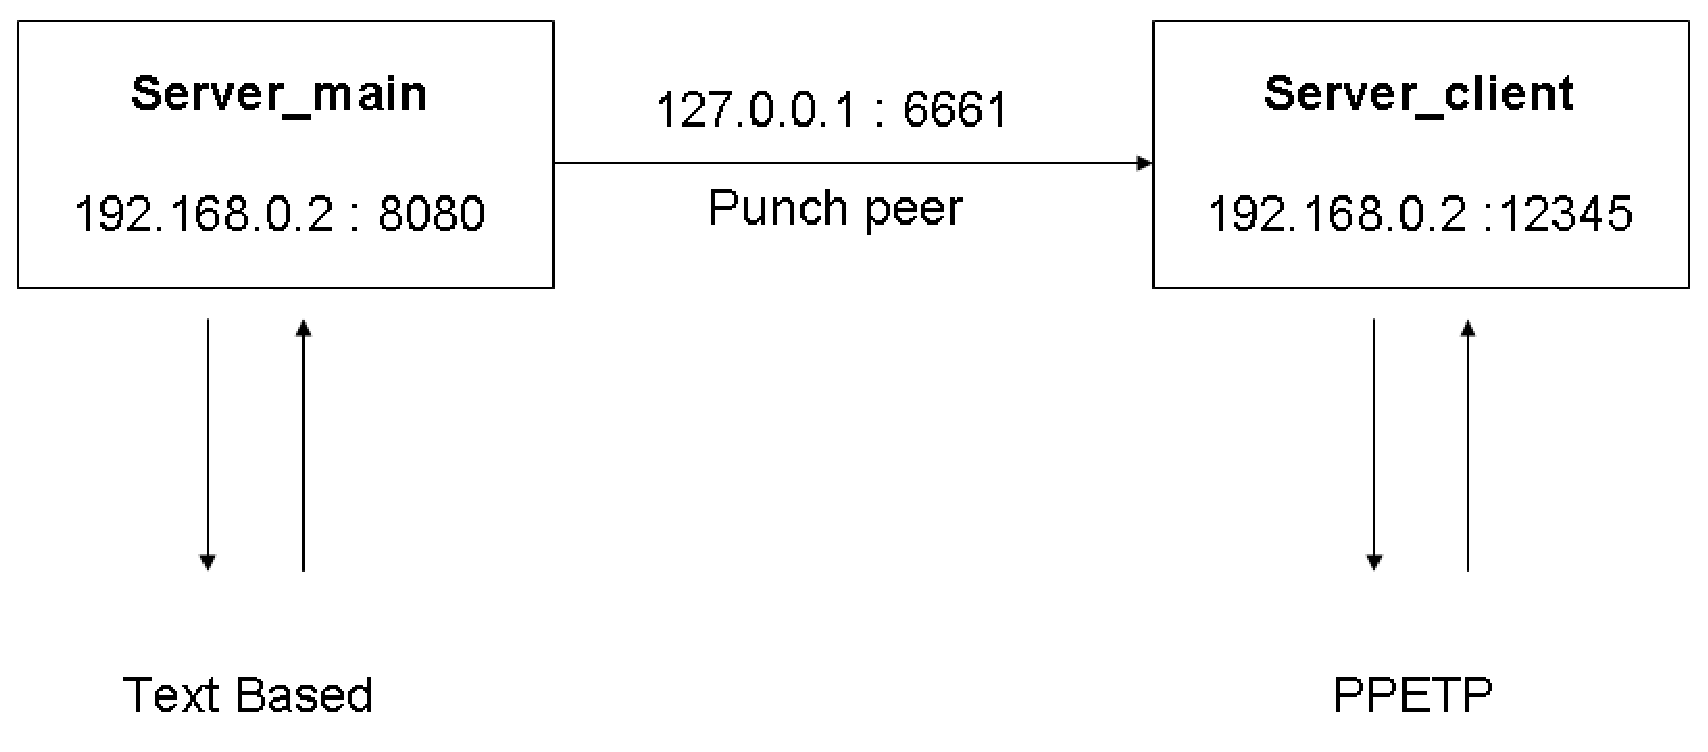
\includegraphics[scale=0.4]{server_structure.eps}
	\caption[Server structure]{Server structure}	
	\label{fig:server_structure}
\end{figure}
%
%**************************************************************************************************
%
\subsection{Testbed configuration}
\label{sec:testbed_configuration}
If you use the same addresses of the figures on the previous section, very little (or none) changes must be done on the scripts. They depend by the hardware/software configuration that you use for the testbed.
The first thing you must grant is that the Control VM can access the others with \emph{ssh} as root\footnote{With the exchange of certificates you can use ssh without provide password. This is recommended; in this way you can launch the simulation script without any other operations}. Once checked that ssh works correctly you must set in the \emph{nat\_traversing\_simultation.sh, execute\_server.sh, execute\_client.sh and execute\_client\_test.sh}, the working directory variable as the root home that must be the same on all the VMs.
After this you must configure the \emph{Peer\_NAT} VM setting the NAT as the default gateway for the ``public'' net. To do this you can modify the network configuration file\footnote{Usually \emph{/etc/network/interfaces}} for automatically add the route otherwise use the command:
\begin{verbatim}
	route add -net 192.168.0.0 netmask 255.255.255.0 gw 192.168.1.2 dev eth0
\end{verbatim}
take attention setting the right \emph{dev} and NAT address.

The configuration of the NAT is quite simple; if you use the sames addresses you must only check the 5th line of the \emph{nat\_config.sh} file to be sure that the \emph{dev} parameter of the \emph{route} command is correct.